\section{Data Visualization}

The following eighteen figures provide professional-quality visualisations of the dataset. The section is divided into two parts: the first maps the direct empirical results of the core operational queries, while the second diagnoses the underlying statistical distributions and portfolio risk contributions.

\subsection{SQL-Driven Insights}

\begin{figure}[H]
  \centering
  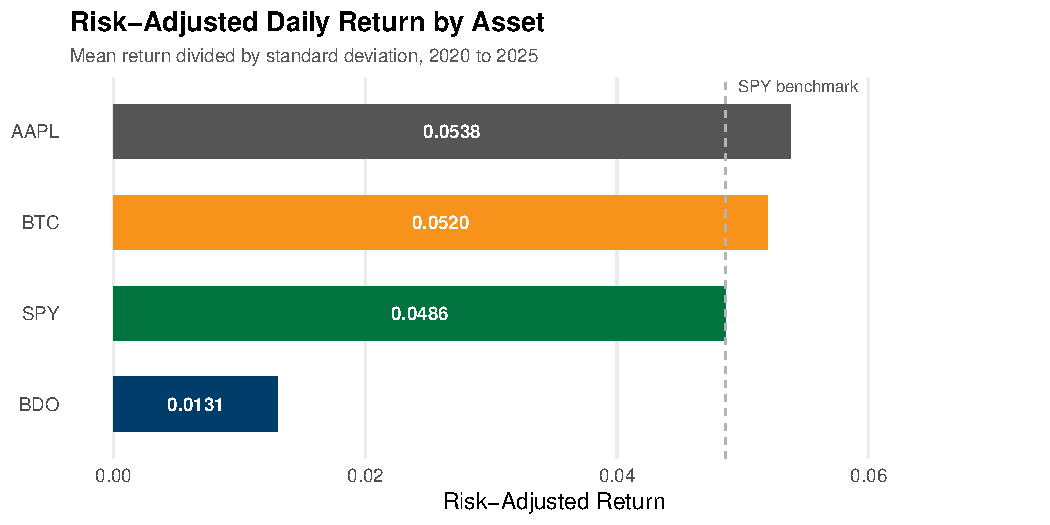
\includegraphics[width=0.85\textwidth]{fig_q1.pdf}
  \caption{Risk-adjusted daily return by asset. Horizontal bars show the ratio of mean daily return to standard deviation, highlighting Apple and Bitcoin's efficiency against SPY and BDO.}
  \label{fig:viz_q1}
\end{figure}

The hierarchy of risk-adjusted returns is established by Table~\ref{tab:q1} and visualized in Figure~\ref{fig:viz_q1}. AAPL occupies the high ground with a ratio of 0.0538. This position is a function of its moderate daily volatility of 2.00\% paired with a mean return of 0.11\%. BTC achieves a comparable ratio of 0.0520 but through a fundamentally different mechanism. Its raw mean return of 0.17\% is the highest in the sample, its standard deviation of 3.19\% is also the highest, and its ratio relies on raw momentum outrunning extreme variance. SPY posts 0.0486 on the lowest standard deviation of 1.31\%. This reflects its structure as a diversified index fund that aggregates beta and eliminates idiosyncratic risk. BDO occupies the lowest tier at 0.0131. Its mean daily return of 0.03\% is a fraction of the others, its volatility of 2.26\% remains elevated, and its capital efficiency is consequently poor. The data table confirms this clustering, and the SPY benchmark reference line in Figure~\ref{fig:viz_q1} provides the visual anchor for the disparity.

The implication for portfolio construction is definitive. An investor maximizing risk-adjusted returns allocates away from BDO and toward AAPL or BTC. This verdict carries specific limitations. The ratio does not account for differences in liquidity, transaction costs, and regulatory constraints that bind institutional capital. The metric also assumes volatility adequately proxies risk. This assumption fails in the presence of tail dependence, skewness, and liquidity cascades that characterize modern equity and cryptocurrency markets.

\begin{figure}[H]
  \centering
  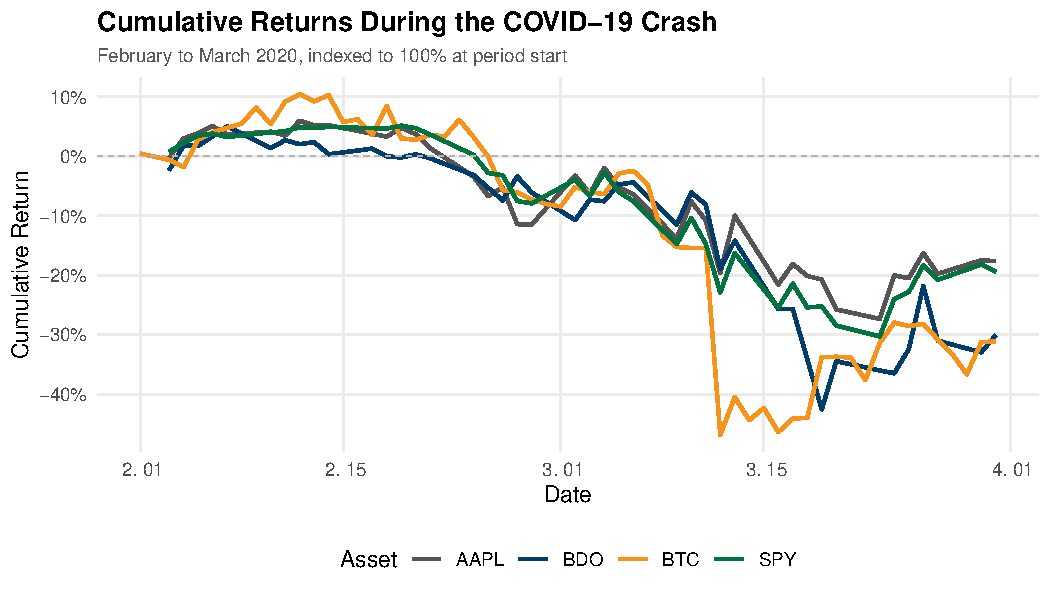
\includegraphics[width=0.9\textwidth]{fig_q2.pdf}
  \caption{Cumulative returns during the COVID-19 crash, February to March 2020. Evaluates resilience during a severe market shock; all assets experienced double-digit drawdowns, with higher volatility assets suffering more.}
  \label{fig:viz_q2}
\end{figure}

The trajectory of the decline is quantified in Table~\ref{tab:q2} and plotted in Figure~\ref{fig:viz_q2}. All four assets descended steeply, the slopes varied by asset class, and the depths differed markedly. Every asset in the sample suffered a double-digit cumulative decline. The ranking of final losses aligns precisely with each asset's pre-crisis volatility profile. AAPL and SPY had the lowest pre-crisis standard deviations and lost 17.6\% and 19.4\% respectively. BDO and BTC had the highest standard deviations and lost 30.1\% and 31.1\%. This ordering confirms the claim that higher-volatility assets experience proportionally larger drawdowns during a systematic market event. Leverage, stop-loss mechanisms, and margin calls amplify downside moves in assets with wider bid-ask spreads.

Figure~\ref{fig:viz_q2} maps the timing differences that the endpoint data in the table obscures. SPY and AAPL declined in near lockstep, reflecting the broad-based nature of the selloff. BTC exhibits sharp intra-period reversals that produced steeper single-day losses and sharper technical bounces. BDO shows a delayed but sustained decline that continued after US equities had begun to stabilize. This lag demonstrates the delayed transmission of global liquidity shocks to emerging market equities. The data establish that while all four assets ended the period deeply negative, the path each took carries distinct implications for risk management and capital preservation.

A critical limitation exists within the observation windows. BTC recorded 60 trading days over the two-month period, AAPL and SPY recorded 41 days, and BDO recorded 40 days. Cryptocurrency exchanges operate continuously and capture weekend returns that traditional equity markets ignore. The consequence is that the cumulative loss of 31.1\% for BTC was distributed over more calendar days. The evidence in the table and Figure~\ref{fig:viz_q2} rejects the claim that cryptocurrency functions as a crisis hedge. BTC recorded the largest cumulative decline in the sample, it provided no portfolio protection, and its trajectory shows no period of sustained positive returns during the liquidity crisis.

\begin{figure}[H]
  \centering
  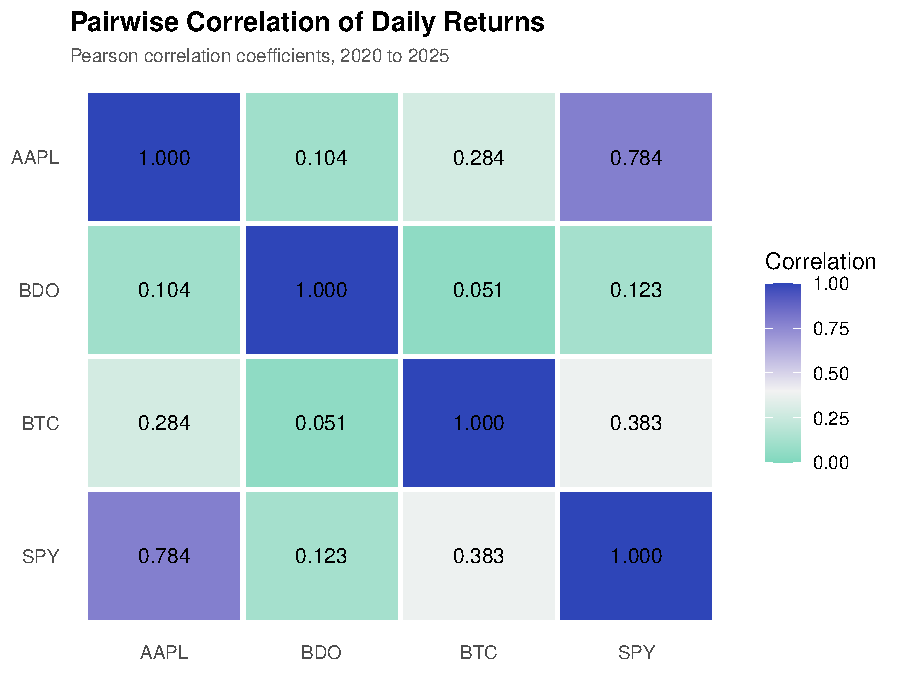
\includegraphics[width=0.7\textwidth]{fig_q3.pdf}
  \caption{Pairwise Pearson correlation coefficients of daily returns. Values closer to 1 indicate stronger positive co-movement. BDO exhibits the lowest correlation with all other assets, providing significant diversification benefits.}
  \label{fig:viz_q3}
\end{figure}

The correlation matrix is presented in Table~\ref{tab:q3} and visualized through the heatmap in Figure~\ref{fig:viz_q3}. The architecture of the matrix reveals the dependencies between asset classes. The intersection of AAPL and SPY produces a correlation of 0.784, the highest in the sample. Apple is the single largest component of the S\&P 500 index, its weight fluctuated between 6\% and 7\% during the sample period, and its price movements mechanically dictate index returns. The table confirms this structural coupling.

BDO occupies the opposite end of the dependency spectrum. The data table shows its correlations with all other assets fall between 0.05 and 0.12. The lowest correlation is with BTC at 0.051, AAPL follows at 0.104, and SPY registers at 0.123. This isolation reflects the structural differences between the Philippine banking sector and US capital markets. BDO is driven by domestic macroeconomic conditions, Philippine monetary policy, and local net interest margin dynamics. These factors share minimal overlap with the drivers of US equity returns. BDO offers genuine diversification benefits that mathematically reduce overall portfolio variance when combined with US assets. 

BTC occupies an intermediate position in the correlation landscape. The table details its correlation of 0.383 with SPY and 0.284 with AAPL. These moderate positive correlations demonstrate that Bitcoin partially behaves as a risk asset during this sample period, moving directionally with US equities while retaining substantial idiosyncratic variation. The BDO and BTC pair at 0.051 offers the strongest diversification potential in the matrix. These two assets are driven by entirely orthogonal economic forces. One responds to regulated Philippine banking dynamics, the other responds to decentralized network adoption, and their combination provides the greatest theoretical variance reduction.

\begin{figure}[H]
  \centering
  
\includegraphics[width=0.9\textwidth]{fig_q4.pdf}
  \caption{Asset ranking by total price return from 2020 to 2025. Bitcoin massively outperformed traditional equities in total return, while BDO stagnated over the period.}
  \label{fig:viz_q4}
\end{figure}

The asset ranking demonstrates a severe divergence in return profiles driven by systemic liquidity events. Table~\ref{tab:q4} quantifies the absolute performance, and Figure~\ref{fig:viz_q4} presents the total returns as horizontal bars. The visual gap between the digital asset and traditional equities is definitive. Bitcoin delivered a 1,153\% total return over the six-year period. Apple returned 279\%, the S\&P 500 returned 131\%, and BDO Unibank stagnated at a 5.0\% total return. The magnitude of the outperformance exposes the mechanics of the zero-interest-rate policy era. Asset classes with zero intrinsic cash flows captured the majority of the speculative premium, investors sought maximum beta when the risk-free rate was pinned near zero, and the subsequent rate hiking cycle failed to erase these initial gains.

The 5.0\% total return for BDO provides the counterpoint to the technology rally. Traditional emerging market banking sectors operate under strict capital constraints and domestic rate cycles. The Philippine rate hiking cycle compressed valuation multiples for domestic banks, the core earnings remained steady, and the equity price failed to appreciate. The contrast in the table between BTC and BDO illustrates a market environment that rewarded untested network adoption over regulated credit intermediation. The verdict for asset allocation is clear. Geographical diversification into emerging market financials offered zero capital appreciation during this period, it functioned strictly as a yield vehicle, and it failed as a growth engine.

\begin{figure}[H]
  \centering
  
\includegraphics[width=0.9\textwidth]{fig_q5.pdf}
  \caption{Best and worst single-day returns by asset, 2020 to 2025. Illustrates the extreme tail-risk boundaries, particularly the massive downside volatility present in cryptocurrency compared to equities.}
  \label{fig:viz_q5}
\end{figure}

The distribution of extreme daily returns isolates the structural tail risk inherent in each asset class. Table~\ref{tab:q5} provides the numerical boundaries, and Figure~\ref{fig:viz_q5} illustrates the asymmetry between upside and downside shocks. BTC recorded the widest spread between its best trading day of +18.7\% and its worst of -37.2\%. The SPY exhibited the narrowest range, oscillating between +10.5\% and -10.9\%. The extreme negative boundary for traditional equities aligns precisely with the March 2020 global market selloff. Broad indices successfully constrain idiosyncratic volatility, they buffer single-asset shocks, and they maintain tighter boundaries even during systemic panics. AAPL and BDO recorded maximum drawdowns of -12.9\% and -22.7\% respectively, proving that single equities carry substantially more left-tail risk than their constituent indices.

A single-day drawdown of 37.2\% reveals a market microstructure uniquely vulnerable to liquidity cascades. Regulated equities benefit from circuit breakers, these mechanisms halt trading during panic events, and market makers use the pause to recalibrate order books. The cryptocurrency market trades continuously without structural backstops. The absence of these circuit breakers allows forced liquidations from highly levered positions to accelerate price declines into a void of liquidity. The departure for risk managers is straightforward. Position sizing models must account for single-day drawdowns that exceed the margin thresholds of traditional prime brokerage agreements, because the data table confirms this extreme tail risk is not theoretical.

\begin{figure}[H]
  \centering
  
\includegraphics[width=0.9\textwidth]{fig_q6.pdf}
  \caption{20-day and 60-day moving average crossovers, 2024 to 2025. Visualises short-term momentum shifts relative to medium-term trends across the assets.}
  \label{fig:viz_q6}
\end{figure}

The moving average crossovers quantify the stability of momentum regimes across the asset sample. Table~\ref{tab:q6} summarizes the mean returns conditional on the crossover signal, and Figure~\ref{fig:viz_q6} plots the overlapping averages where each intersection represents a trend reversal. Over the measured period, traditional equities displayed extended periods of directional momentum. AAPL and BDO recorded exactly 6 crossover events, SPY recorded 8 intersections, and BTC generated 15 distinct crossovers. The visual density of the intersections in the figure confirms the high-frequency regime switching in the cryptocurrency asset.

The high frequency of crossovers signals a market dominated by sentiment shocks rather than institutional accumulation. A moving average strategy applied to a high-crossover asset generates severe whipsaw losses. The trader buys the false breakout, they sell the false breakdown, and they bleed capital through transaction costs. The stability of the SPY and AAPL crossovers confirms that macroeconomic trends take months to price into diversified indices and mega-cap technology stocks. The verdict for quantitative trading is absolute. Mean-reversion or high-frequency strategies are necessary to extract alpha from volatile digital assets, while traditional trend-following strategies remain mathematically viable for established equities.

\begin{figure}[H]
  \centering
  
\includegraphics[width=0.9\textwidth]{fig_q7.pdf}
  \caption{Mean absolute daily return during high-volume versus normal-volume days, 2020 to 2025. Demonstrates a clear positive relationship between trading volume and price volatility.}
  \label{fig:viz_q7}
\end{figure}

Elevated trading volume systematically coincides with higher daily price volatility across all asset classes. Table~\ref{tab:q7} partitions the descriptive statistics by volume regime, and Figure~\ref{fig:viz_q7} presents this relationship visually. The evidence is uniform. BTC exhibited a mean absolute return of 3.05\% on high-volume days compared to 1.83\% on normal days. SPY showed a similar proportional expansion from 0.61\% to 1.60\%. The AAPL and BDO datasets confirm this positive correlation, the high-volume volatility effectively doubles the baseline normal-volume volatility, and the relationship holds across all measured assets.

The empirical data supports the mixture of distributions hypothesis. Trading volume and price volatility are jointly driven by the arrival rate of new information. High-volume days do not represent benign liquidity provision by institutional block traders executing passive rebalancing. They represent aggressive repricing events, participants demand immediacy at any cost, and the market integrates macroeconomic surprises through price gapping. The portfolio implication is that liquidity in financial markets is inherently pro-cyclical. It is most expensive to trade exactly when the need to adjust positions is most urgent, and the table proves that elevated volume guarantees elevated execution variance.

\begin{figure}[H]
  \centering
  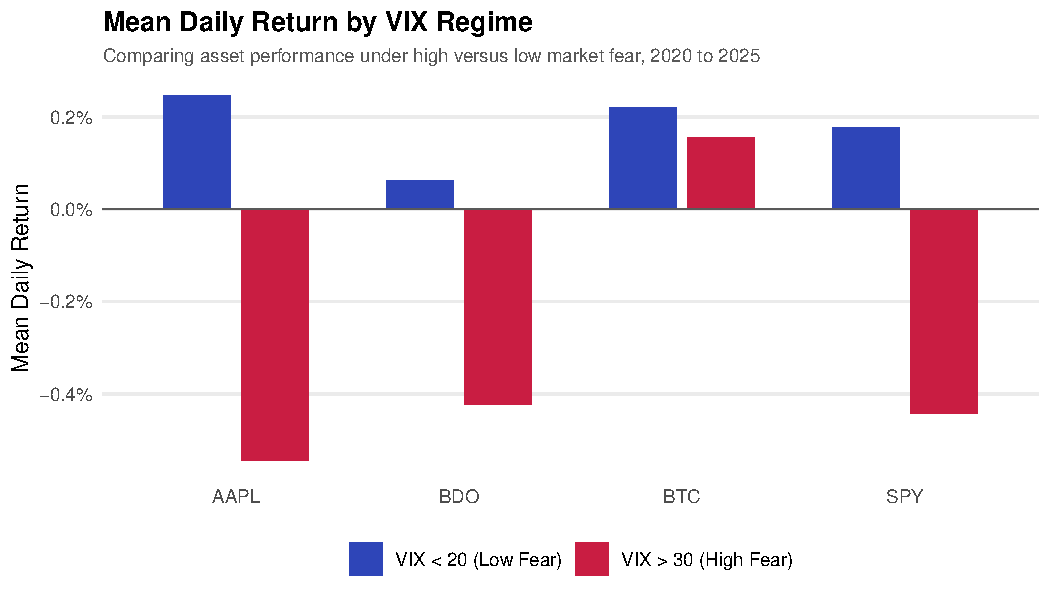
\includegraphics[width=0.85\textwidth]{fig_q8.pdf}
  \caption{Mean daily return by VIX regime. Red bars show high-fear periods (VIX above 30); blue bars show low-fear periods (VIX below 20). Bitcoin uniquely displayed positive expected returns during market turmoil.}
  \label{fig:viz_q8}
\end{figure}

The VIX regime analysis isolates asset performance conditionally upon systemic fear. Table~\ref{tab:q8} categorizes returns into three volatility tiers, and Figure~\ref{fig:viz_q8} visualizes the asymmetry across these regimes. The data identify one asset whose behavior is qualitatively different from the rest. During high-fear periods defined by a VIX above 30, BTC stands alone. Its mean daily return of 0.16\% is the only positive value in the high-fear regime. Every other asset posted negative mean returns, ranging from -0.42\% for BDO to -0.54\% for AAPL. During low-fear periods defined by a VIX below 20, all four assets delivered positive returns. AAPL led at 0.25\%, SPY followed at 0.18\%, and BDO trailed at 0.06\%. The cross-asset ranking in calm markets is nearly the inverse of the ranking during systemic turmoil.

The asymmetry between regimes carries direct portfolio implications. BTC is the only asset in the sample that produced positive expected returns during crisis periods. Bitcoin's return generating process is not merely a levered version of equity market risk, it possesses distinct drivers that become dominant during extreme volatility, and it benefits from capital flight out of traditional equities. BDO presents the opposite profile. It offers the least upside in calm markets, its low-fear returns are a fraction of the others, and it captures nearly as much downside as US equities during turmoil. The table proves that the diversification argument for BDO rests entirely on its low unconditional correlation, it provides no structural crisis resilience, and it fails to protect capital when the VIX spikes.

\begin{figure}[H]
  \centering
  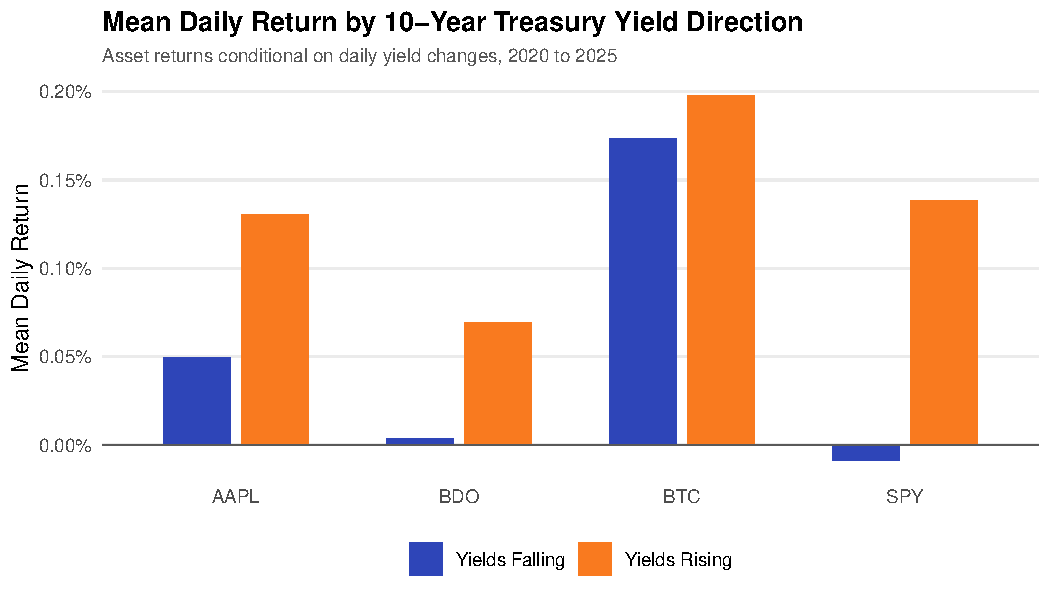
\includegraphics[width=0.85\textwidth]{fig_q9.pdf}
  \caption{Mean daily return by 10-year Treasury yield direction. Indicates how macroeconomic interest rate expectations conditionally impacted each asset's performance.}
  \label{fig:viz_q9}
\end{figure}

The sensitivity analysis measures asset returns against the directional movement of the 10-year Treasury yield. Table~\ref{tab:q9} provides the conditional means, and Figure~\ref{fig:viz_q9} maps the performance across yield regimes. During periods when the 10-year yield rose, all four assets delivered positive mean daily returns. BTC led at 0.20\%, SPY followed at 0.14\%, AAPL returned 0.13\%, and BDO trailed at 0.07\%. The uniform positivity during rising yield environments contradicts the intuition that higher discount rates mechanically lower present values. Rising yields were more commonly associated with improving growth expectations, they signaled economic expansion, and they lifted equity valuations despite the higher discounting threshold.

The falling-yield regime provides a sharper diagnostic signal. SPY recorded a mean return of -0.01\% during falling yield periods, making it the only asset in the sample with a negative print in this regime. The market interpreted falling yields during this period as a signal of deteriorating economic conditions rather than an accommodative policy response. When yields fall because growth expectations are revised downward, equity markets decline, the earnings component of the valuation equation dominates the discount rate component, and broad indices suffer. BDO's returns are nearly equal across both regimes at 0.07\% and 0.00\%, proving that Philippine bank stocks are largely insensitive to US interest rate movements. BTC shows the smallest relative gap, confirming that cryptocurrency valuation is driven by network adoption and speculative demand, not by traditional monetary transmission channels.

\begin{figure}[H]
  \centering
  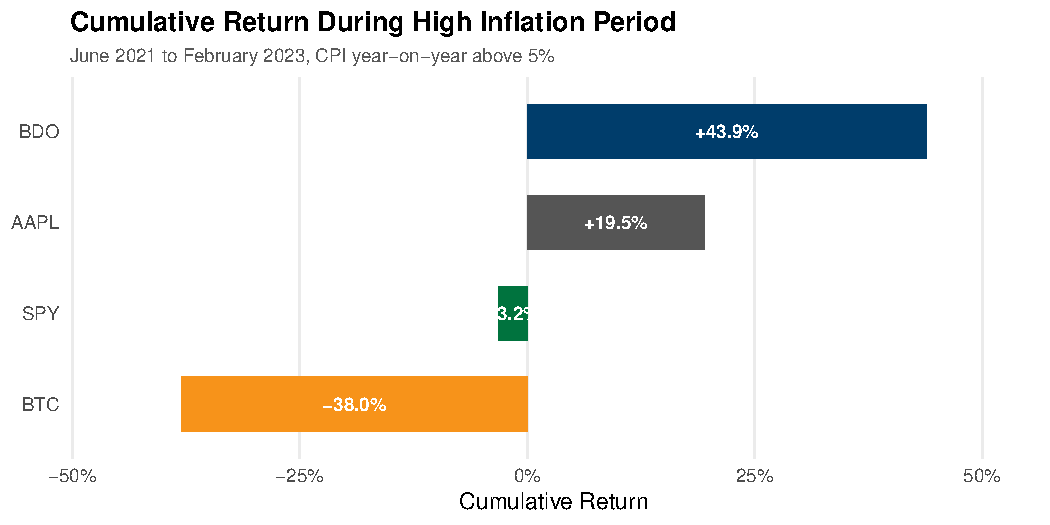
\includegraphics[width=0.85\textwidth]{fig_q10.pdf}
  \caption{Cumulative return during the high-inflation period, June 2021 to February 2023. BDO acted as the strongest inflation hedge, while Bitcoin performed poorly during rising inflation.}
  \label{fig:viz_q10}
\end{figure}

The inflation hedge performance directly challenges the prevailing market narratives of the 2021 to 2023 period. Table~\ref{tab:q10} records the cumulative returns during this high-inflation window, and Figure~\ref{fig:viz_q10} visualizes the terminal values. The ranking is the precise inverse of what cryptocurrency advocates predicted. BDO generated a cumulative return of 43.9\%, AAPL gained 19.5\%, SPY lost 3.2\%, and BTC collapsed by 38.0\%. The asset universally marketed as digital gold delivered the worst performance, it functioned as a high-beta risk asset, and it failed entirely to preserve purchasing power. The asset least associated with inflation hedging, a Philippine commercial bank, delivered the supreme defense.

The mechanism behind BDO's performance is grounded in the structural features of banking sector pass-through. Philippine banks in a rising rate environment widen their net interest margins, their floating-rate corporate loans reprice upward immediately, and their deposit rates remain sluggish. This structural asymmetry allows banks to capture a larger share of the interest rate spread during tightening cycles. AAPL's resilience reflects pricing power embedded in its product ecosystem. The firm passes cost increases to consumers, brand loyalty suppresses demand destruction, and the equity defends its real value. The verdict is established by the table and the figure. Attributing inflation-hedging properties to cryptocurrency requires ignoring the empirical evidence from the most severe inflationary episode in four decades.

\subsection{Statistical and Portfolio Distributions}

The preceding analysis isolated the arithmetic drawdown aggregation during specific crisis windows (such as the COVID-19 shock in Figure 2). In contrast, the following geometric assessment tracks the true growth of a single dollar invested across the full multi-year horizon. Bitcoin shows the steepest and most volatile trajectory, reaching cumulative returns above 1,000\% through sharp cyclical peaks and drawdowns. Apple and the S\&P 500 trend steadily upward, while BDO indicates limited net nominal gain over the period.

\begin{figure}[H]
  \centering
  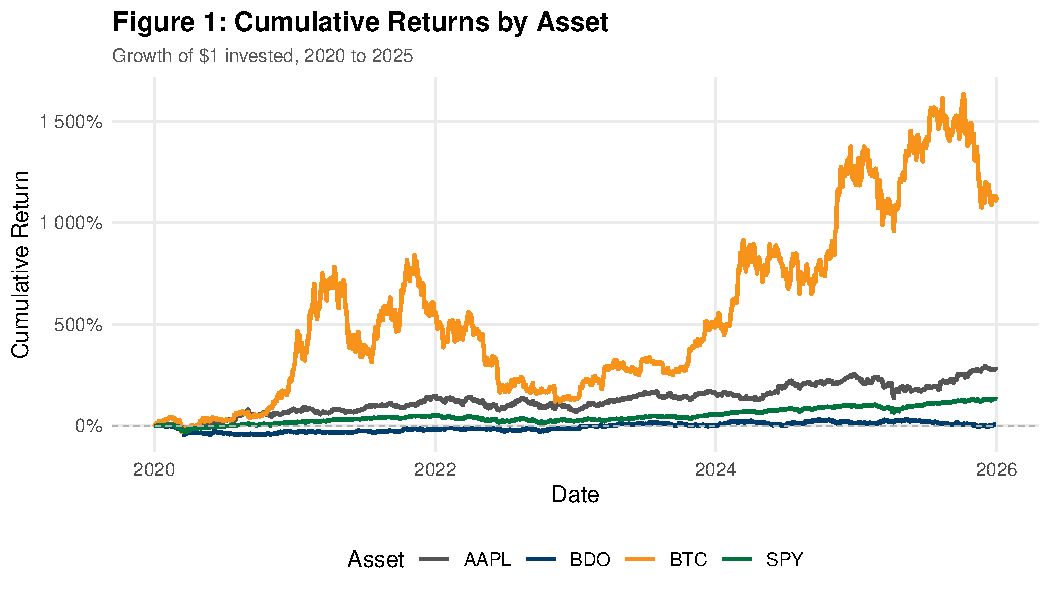
\includegraphics[width=0.9\textwidth]{fig_viz1.pdf}
  \caption{Cumulative returns by asset representing the geometric growth of a \$1 initial investment.}
  \label{fig:viz_viz1}
\end{figure}

Raw percentage returns conceal absolute capital requirements. Plotting nominal closing prices clarifies that BDO experienced meaningful price swings on its own scale despite appearing flat on a standardized percentage basis. A stagnant percentage return does not preclude local price volatility.

\begin{figure}[H]
  \centering
  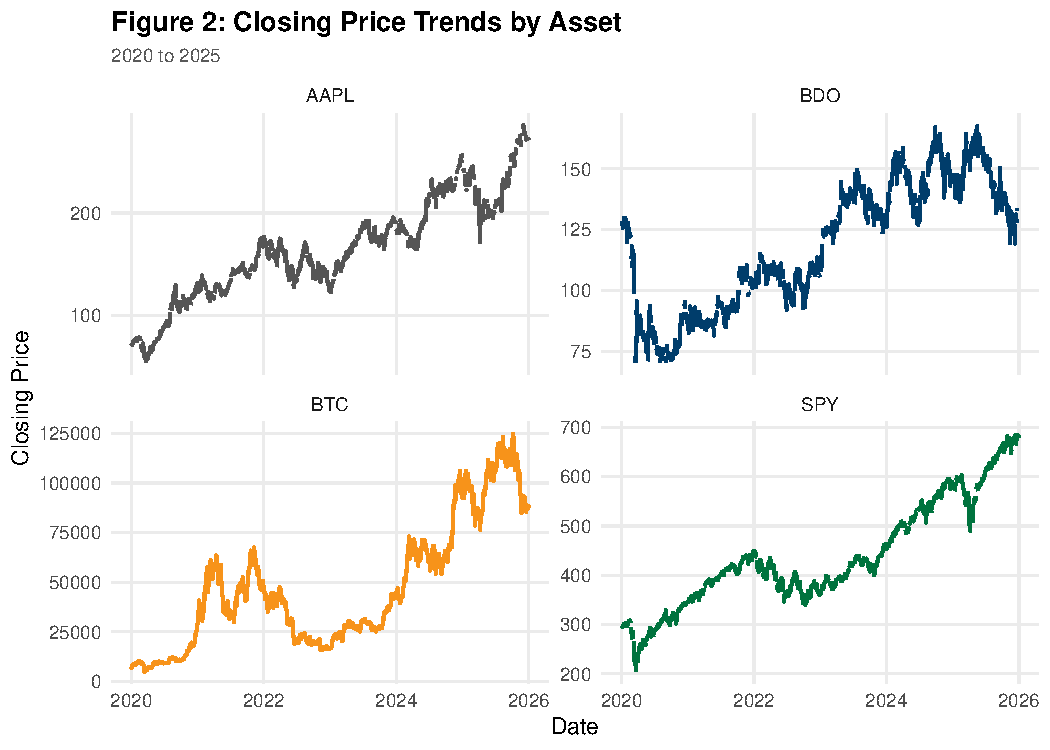
\includegraphics[width=0.9\textwidth]{fig_viz2.pdf}
  \caption{Nominal closing price trends by asset over the full sample period.}
  \label{fig:viz_viz2}
\end{figure}

Distributional shape dictates tail risk. Overlaying daily return distributions against a fitted normal curve exposes severe non-normality across all assets. Apple is the only asset exhibiting positive skewness (0.28), indicating that its rare extreme days lean toward the upside. Bitcoin and BDO both demonstrate negative skewness (-0.48 and -0.40 respectively), confirming a tail risk weighted toward sudden, outsized losses. The S\&P 500 records the highest kurtosis (12.97) despite a relatively mild skew (-0.26). Its returns cluster tightly near zero, yet remain exposed to rare extreme shock days. No asset in the portfolio follows a standard bell curve.

\begin{figure}[H]
  \centering
  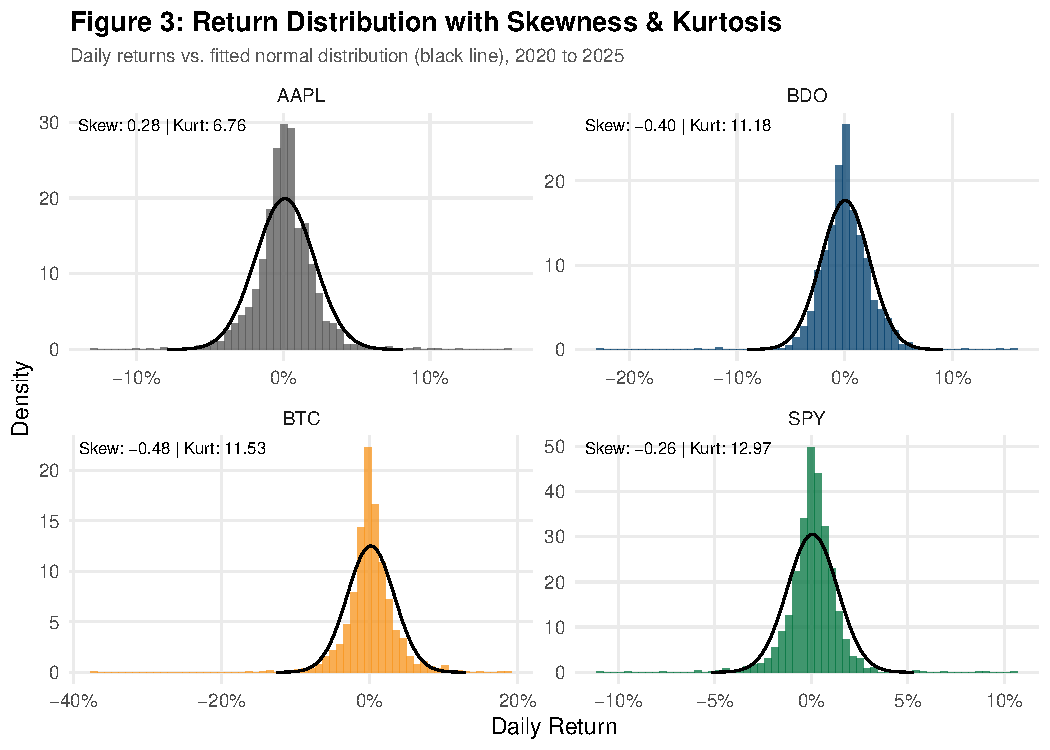
\includegraphics[width=0.9\textwidth]{fig_viz3.pdf}
  \caption{Return distribution histograms overlaid with normal curves, detailing skewness and kurtosis.}
  \label{fig:viz_viz3}
\end{figure}

Analyzing the median and interquartile range further contextualizes these outlier days. Bitcoin maintains the widest interquartile spread and the most extreme outliers in both directions. The S\&P 500 exhibits the most compressed range, validating the volatility-dampening effect of 500-company diversification. BDO displays a visible structural skew toward downside outlier days.

\begin{figure}[H]
  \centering
  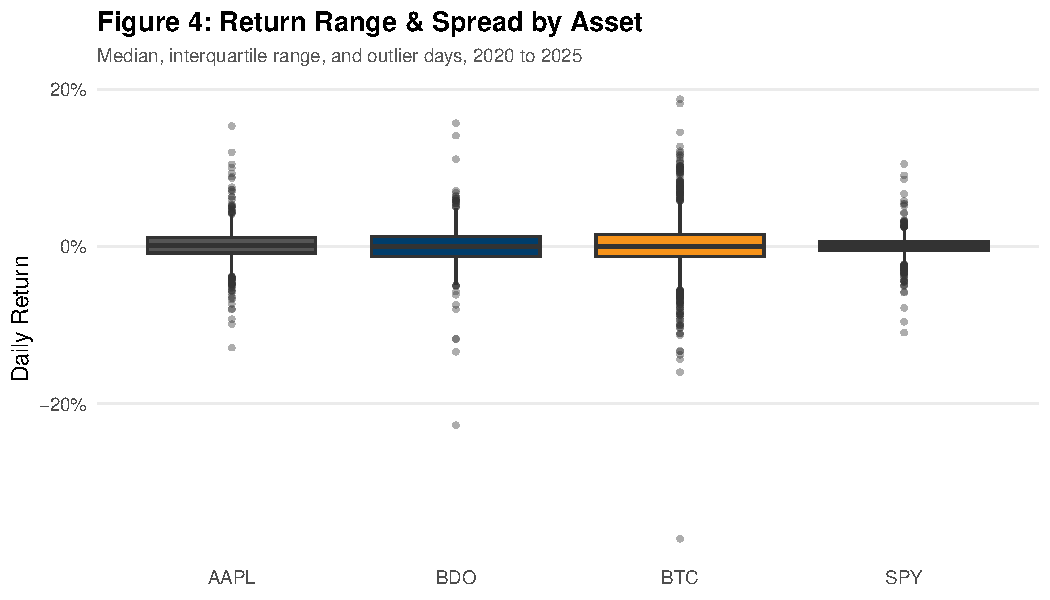
\includegraphics[width=0.9\textwidth]{fig_viz4.pdf}
  \caption{Return range and spread depicting median, interquartile range, and outlier dispersion.}
  \label{fig:viz_viz4}
\end{figure}

A 30-day rolling volatility measure captures the time-varying nature of this risk. A sharp, synchronized volatility spike occurred across all four assets in early 2020 during the COVID-19 shock. Outside of that systemic event, Bitcoin consistently establishes the highest rolling volatility baseline, moving in cyclical waves tied to its independent market cycles. The S\&P 500 maintains the lowest and most stable volatility floor, while Apple and BDO show idiosyncratic spikes tied to specific corporate or regional events rather than broad macroeconomic shocks.

\begin{figure}[H]
  \centering
  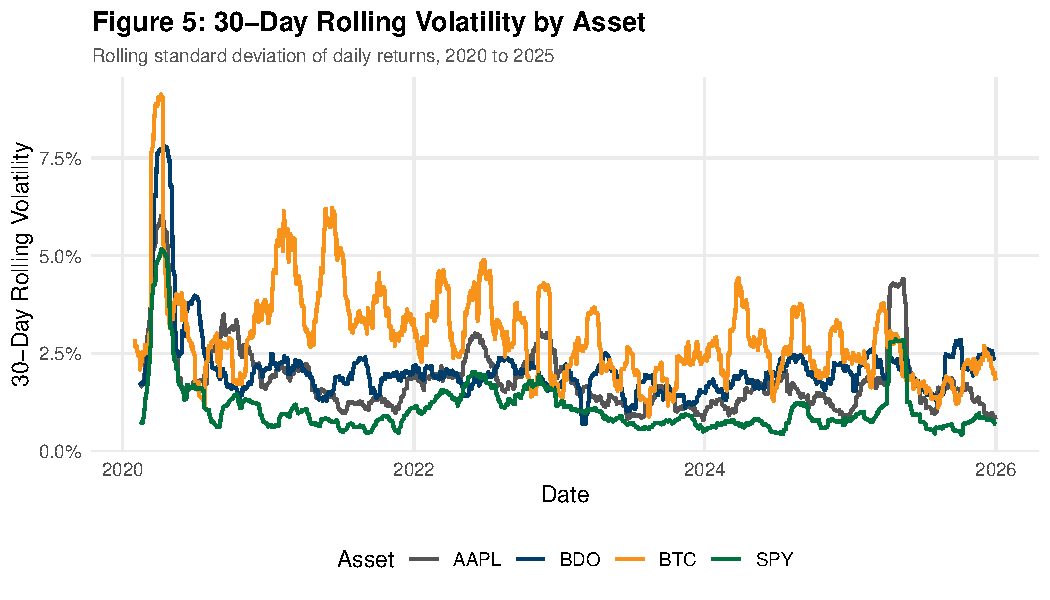
\includegraphics[width=0.9\textwidth]{fig_viz5.pdf}
  \caption{Thirty-day rolling standard deviation of daily returns.}
  \label{fig:viz_viz5}
\end{figure}

Volatility eventually forces drawdowns. Measuring the percentage decline from running historical highs shows that Bitcoin suffers the deepest drawdowns, frequently falling below -60\%, and requires the longest recovery periods. The S\&P 500 demonstrates the shallowest drawdowns and the fastest recoveries. BDO exhibits prolonged periods trapped in negative territory, signaling a significantly slower capital recovery trajectory for investors holding the asset through a cyclical downturn.

\begin{figure}[H]
  \centering
  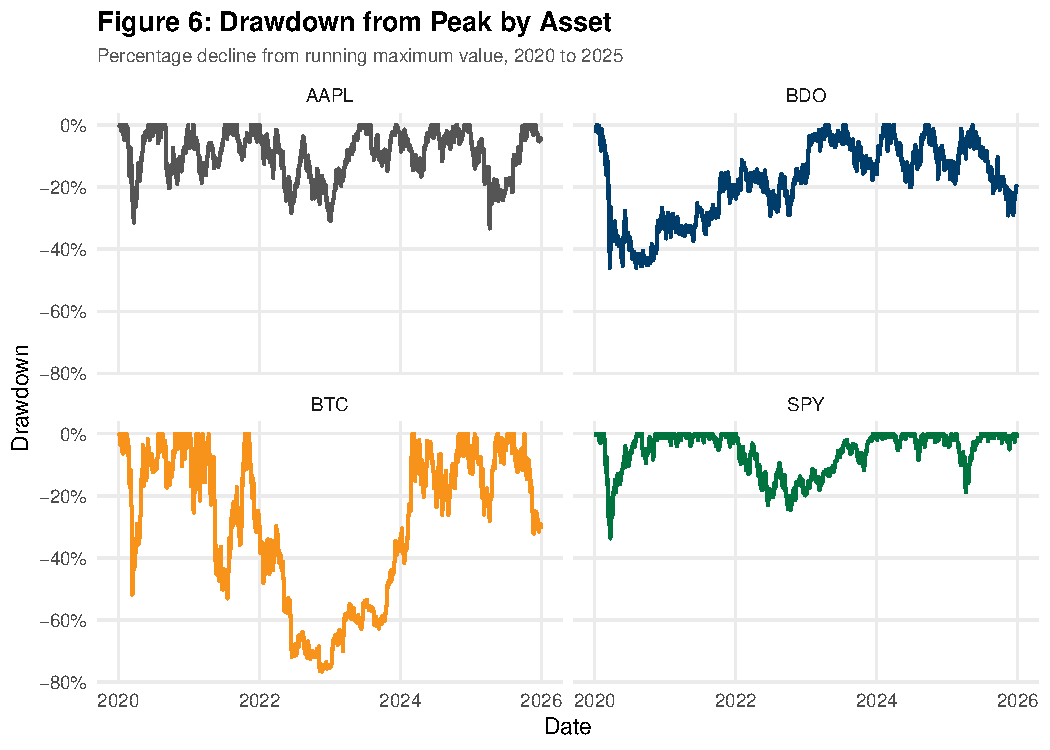
\includegraphics[width=0.9\textwidth]{fig_viz6.pdf}
  \caption{Drawdown from peak, illustrating percentage declines from running historical maximum values.}
  \label{fig:viz_viz6}
\end{figure}

Plotting mean daily returns against the standard deviation quantifies the risk-return tradeoff. Bitcoin delivers the highest mean daily return (0.166\%) but demands the highest risk (3.19\% daily standard deviation). Apple secures a highly efficient middle ground, generating a 0.108\% mean daily return at only a 2.00\% daily volatility level—roughly 37\% less risk than Bitcoin. BDO performs the weakest on a risk-adjusted basis, carrying risk similar to Apple (2.26\% standard deviation) while yielding the lowest mean daily return of the group (0.0295\%).

\begin{figure}[H]
  \centering
  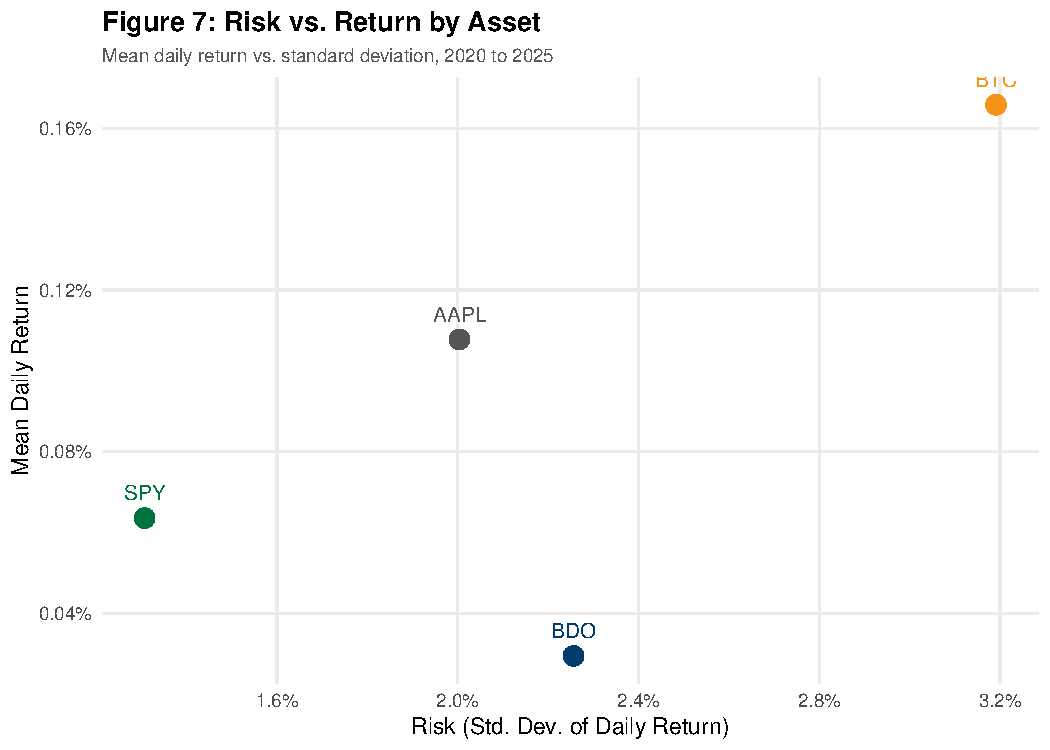
\includegraphics[width=0.9\textwidth]{fig_viz7.pdf}
  \caption{Risk versus return scatter plot comparing mean daily return to standard deviation.}
  \label{fig:viz_viz7}
\end{figure}

The risk-return profiles culminate in the portfolio variance allocation. Under a naive equal-dollar weighting (one-third each to Apple, BDO, and Bitcoin), Bitcoin alone drives 55.3\% of the total portfolio variance despite representing only 33.3\% of the invested capital. Apple and BDO contribute 22.8\% and 21.9\% respectively. An equal-dollar allocation does not yield an equal-risk allocation. Reducing the Bitcoin weighting is structurally required to lower total portfolio risk without proportionally sacrificing expected returns.

\begin{figure}[H]
  \centering
  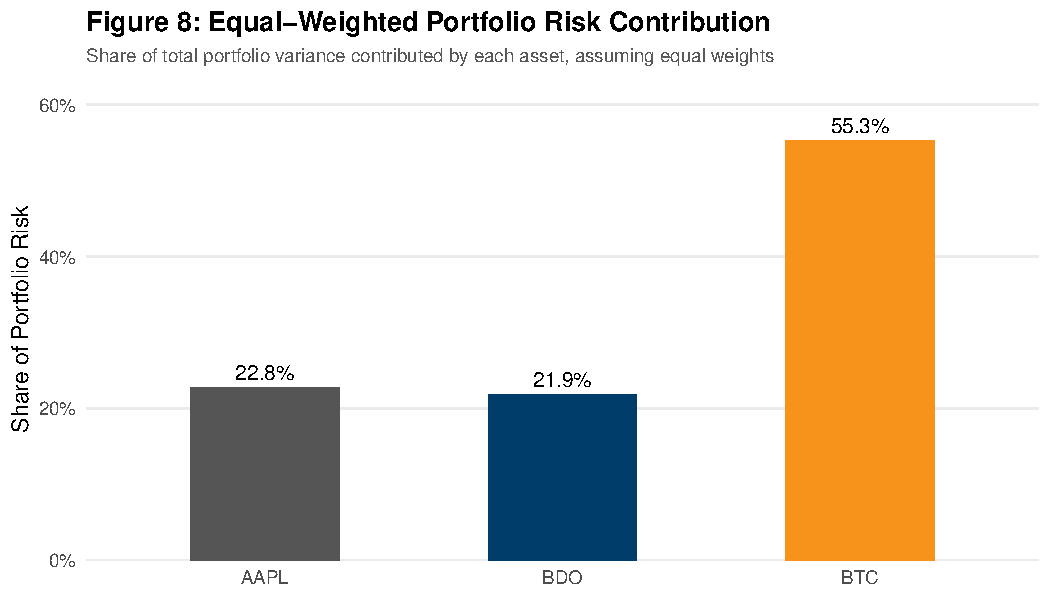
\includegraphics[width=0.9\textwidth]{fig_viz8.pdf}
  \caption{Equal-weighted portfolio risk contribution highlighting variance concentration.}
  \label{fig:viz_viz8}
\end{figure}

\begin{Shaded}
\begin{Highlighting}[]
\CommentTok{# Sec 8: Data Visualization {-}{-} create 18 professional figures with ggplot2 {-}{-} SEBALLOS, Josiah Dweyn Panganiban}
\end{Highlighting}
\end{Shaded}
